\documentclass[titlepage,12pt,a4paper]{article}

\usepackage[slovene]{babel}
%\usepackage{color}
\usepackage{graphicx}
%\usepackage{subfigure}
\usepackage{mathtools}
\usepackage{float}
\usepackage{url}

\title{Zaključna naloga : precesija Lunine orbite}

\author{Niko Cabello}

\date{\today}

\begin{document}

\maketitle
%\listoftables
\tableofcontents

\newpage

\section{Uvod}
\label{sec : Uvod}
\subsection{Naloga}
\label{subsec : Naloga}
Namen naloge je raziskati, kako se Lunina orbita spreminja s časom. Ker Lunina orbita ni v isti ravnini kot Zemljina orbita okoli Sonca, pride do stalnega spreminjanja Lunine orbite. Z numeričnim integriranjem simuliramo orbiti Zemlje okoli sonca in Lune okoli Zemlje in opazujemo, kako se Lunina orbita spreminja.

\subsection{Prva podnaloga}
Pri prvi podnalogi opazujemo, kako se kot med ravnino Lunine orbite okoli Zemlje in ravnino Zemljine orbite okoli Sonca spreminja.
\subsection{Druga podnaloga}
Pri drugi podnalogi opazujemo, kako se spreminja položaj velike polosi Lunine orbite okoli Zemlje.
\subsection{Seznam uporabljenih oznak}
\begin{table}[H]
\begin{large}
\renewcommand{\arraystretch}{1.3}
\begin{tabular}{ |c| c || p{8.5cm} | }
 oznaka& enote& pomen\\
 \hline
 \hline
 $\kappa = 6.6743 \times 10^{-11}$& $\frac{Nm^{2}}{kg^{2}}$ & gravitacijska konstanta\\
 $M_S = 1.989 \times 10^{30}$ & $kg$ & masa Sonca \\
 $M_Z = 5.9724 \times 10^{24}$ & $kg$ & masa Zemlje  \\
 $r_{SZ_{min}} = 147.095 \times 10^{9}$ & $m$ & najmanjša razdalja od Sonca do Zemlje \\
 $v_{Z_{min}} = 30.29 \times 10^{3}$ & $\frac{m}{s}$ & Hitrost Zemlje, glede na Sonce, ko je  Zemlja najbližje Soncu \\
 $v_{ZS}$ & $\frac{m}{s}$ & Hitrost Zemlje, glede na Sonce \\
 $M_L = 0.07346 \times 10^{24}$ & $kg$ & masa Lune \\
 $r_{{min}} = 0.3633 \times 10^{9}$ & $m$ & najmanjša razdalja od Zemlje do Lune \\
 $r_{{max}} = 0.4055 \times 10^{9}$ & $m$ & največja razdalja od Zemlje do Lune \\
 $v_{L_{min}}$ & $\frac{m}{s}$ & Hitrost Lune, glede na Zemljo, ko je Luna najbližje Zemlji \\
 $v_{L_{max}}$ & $\frac{m}{s}$ & Hitrost Lune, glede na Zemljo, ko je Luna najbolj oddaljena Zemlji\\
 $v_{LS}$ & $\frac{m}{s}$ & Hitrost Lune, glede na Sonce \\
 $\theta = 5.15$ & ° & Začeten kot med ravnino Lunine orbite okoli Zemlje in ravnino Zemljine orbite okoli Sonca\\
 $\overrightarrow{r_{XY}}$ & $m$ & Vektor od nekega objekta X do nekega objekta Y \\
 \hline
\end{tabular}
\caption{Tabela spremenljivk in njihovi pomeni. Podatki so bili prevzeti iz \cite{Zak nal}, \cite{Luna}, \cite{Zemlja}, \cite{Sonce}}
\end{large}
\end{table}

\section{Teoretični del}
\label{sec : teoreticni del}
\subsection{Teoretična zasnova}
Na vsako ne nabito telo v vesolju deluje le gravitacijska sila. Ker predpostavimo, da so vsi objekti (Luna, Zemlja ...) točkasti, je gravitacijska sila centralna. Silo objekta A na objekt B izračunamo po enačbi (\ref{Grav. sila}),

\begin{large}
\begin{equation}
\overrightarrow{F_{AB}} = -\frac{\kappa\ M_A\ M_B}{|\overrightarrow{{r_{AB}}}|³}\ \overrightarrow{{r_{AB}}} \label{Grav. sila}
\end{equation}
\end{large}

kjer so $M_A$ in $M_B$ masi objektov A in B, $\kappa$ gravitacijska konstanta in $\overrightarrow{r_{AB}}$ vektor od objekta A do objekta B.

\subsection{Pospeški lune}
V našem sistemu na Luno s silo delujeta le dva objekta Zemlja in Sonce.
Zato je pospešek Lune enak vsoti pospeška zaradi Zemlje in pospeška zaradi Sonca. Pospešek Lune zaradi nekega objekta X izračunamo po enačbi (\ref{grav. pospešek}).

\begin{large}
\begin{equation}
\overrightarrow{a_{LX}} = -\frac{\kappa\ M_X}{|\overrightarrow{{r_{XL}}}|³}\ \overrightarrow{{r_{XL}}}  \label{grav. pospešek}
\end{equation}
\end{large}


\subsection{Hitrost Lune}
Ker problem rešujemo z numeričnim integriranjem so pomembni začetni pogoji. Eden od njih je tudi hitrost Lune glede na Zemljo, ki jo lahko izračunamo iz enačbe za ohranitev vrtilne količine in iz enačbe za ohranitev energije.
\\

Enačba za ohranitev vrtilne količine pri točkastih telesih:
\begin{large}
\begin{eqnarray}
r_{min}\ v_{L_{min}} =  r_{max}\ v_{L_{max}} \\
v_{max} = \frac{r_{min}}{r_{max}}\ v_{L_{min}} \label{gib. kol. razm.}
\end{eqnarray}
\end{large}

Enačba za ohranitev energije:
\begin{large}
\begin{align}
W_{k1} + W_{p1} &= W_{k2} + W_{p2}\\
\frac{M_L\ v_{L_{min}}^{2}}{2} - \kappa\ \frac{M_L\ M_Z}{r_{min}} &= \frac{M_L\ v_{L_{max}}^{2}}{2} - \kappa\ \frac{M_L\ M_Z}{r_{max}} \\
v_{L_{min}}^{2} - v_{L_{max}}^{2} &= 2\ \kappa\ M_Z\ \left(-\frac{1}{r_{max}} + \frac{1}{r_{min}} \right) \\
\intertext{$v_{L_{max}}$  zamenjamo z zvezo iz enačbe (\ref{gib. kol. razm.}) in dobimo} 
v_{L_{min}}^{2} &= 2\ \kappa\ M_Z\ \frac{\left(-\frac{1}{r_{max}} + \frac{1}{r_{min}} \right)}{1 - \left(\frac{r_{min}}{r_{max}}\right)^{2}} \label{hitorst v min}
\end{align}
\end{large}

Po enačbi (\ref{hitorst v min}) lahko izračunamo kakšno hitrost ima Luna, ko je najbližje Zemlji.

\subsection{Numerično integriranje}
Numerično integriracijo sem opravil v programskem jeziku Python s pomočjo knjižnice SciPy. Za numerično integriranje je potrebno definirati funkcijo, ki vrne vrednosti ob nekem času $t$, ki jih nato  funkcija solve\_ivp iz knjižnice SciPy pomnoži z nekim majhnim časovnim intervalom $\varDelta t$. Tako dobimo spremembe naših vrednosti ob času $t$. Naša spremembe seštejemo z našimi vrednostmi ob času $t$ in vsoto shranimo. Tako smo dobili vrednost ob času $t + \varDelta t$. Vrednosti, ki sem jih spreminjal v tej funkciji so vektor od Zemlje do Lune ($\overrightarrow{r_{ZL}}$), hitrost Lune glede na Sonce ($\overrightarrow{v_{LS}}$), vektor od Sonca do Zemlje ($\overrightarrow{r_{SZ}}$) in hitrost Zemlje glede na Sonce ($\overrightarrow{v_{ZS}}$). Primer hitrosi Zemlje ob času $t + \varDelta t$:

\begin{large}
$$\varDelta \overrightarrow{v_{ZS}}(t) = \dot{\overrightarrow{v_{ZS}}}(t) \varDelta t $$
$$\varDelta \overrightarrow{v_{ZS}}(t) = \overrightarrow{a_{ZS}}(t) \varDelta t$$
$$\overrightarrow{v_{ZS}}(t + \varDelta t) =  \overrightarrow{v_{ZS}}(t)\ +\ \varDelta\overrightarrow{v_{ZS}}(t)$$
$$\overrightarrow{v_{ZS}}(t + \varDelta t) =  \overrightarrow{v_{ZS}}(t)\ +\ \overrightarrow{a_{ZS}}(t) \varDelta t$$
\end{large}

Pri numeričnem integriranju sem definiral, da je orbita Zemlje okoli Sonca na XY-ravnini.

Za pot, ki jo opravi Luna okoli Zemlje, je pomombno spreminjanje vektorja $\overrightarrow{r_{ZL}}$. Ostale vrednosti so potrebne, da lahko simuliramo Lunino pot v neinercialnem sistemu (osončje). Začetne vrednosti, ki sem jih izbral so :

\begin{large}
\begin{eqnarray}
\overrightarrow{r_{ZL}} &=& \left(0, r_{min}\ cos(\theta), r_{min}\ sin(\theta) \right) \\
\overrightarrow{v_{LS}} &=& \left(v_{L_{min}}, 0, 0\right) + \overrightarrow{v_{ZS}} \\
\overrightarrow{r_{SZ}} &=& \left(0, r_{SZ_{min}}, 0\right) \\
\overrightarrow{v_{ZS}} &=& \left(v_{Z_{min}}, 0, 0 \right) 
\end{eqnarray}
\end{large}

Poleg same integracije poti, sem naredil funkcijo, ki gleda, kdaj Luna prečka YZ-ravnino tako, da ima pred prečkanjem ravnine Luna negativno X-komponento in po prečkanju ravnine pozitivno X-komponento. Sepravi bodo vektorji prečkanja te ravnine oblike $\overrightarrow{r_{p}} = (0,\ y,\ z)$ in glede na začetne pogoje bo $y >= 0$. Interval med dvema takima prečkanjima YZ-ravnine sem definiral kot eno orbito okoli Zemlje. Ker vemo kakšna je Z-komponenta vektorja od Zemlje do Lune, ko prečkamo to ravnino, lahko izračunamo kakšen je kot med ravnino Zemljine orbite okoli Sonca in Luno (kot med XY-ravnino in vektorjem $\overrightarrow{r_{p}}$), ko začne z novo orbito. Kot lahko enostavno izračunamo po enačbi (\ref{kot ravnine XY}).

\begin{large}
\begin{equation}
\alpha = arcsin\left(\frac{\overrightarrow{r_{p}} \cdot \left(0, 0, 1\right)}{|\overrightarrow{r_{p}}|}\right) \label{kot ravnine XY}
\end{equation}
\end{large}

Pri opazovanju, kako se spreminja položaj velike polosi orbite je potrebno razdeliti množico $\{\overrightarrow{r_{ZL}}(t_0),\ \overrightarrow{r_{ZL}}(t_0 + \varDelta t),\ \overrightarrow{r_{ZL}}(t_0 + 2\varDelta t),\ ...\ , \overrightarrow{r_{ZL}}(t_0 + N\varDelta t)\} $ na grupe, kjer so v posamezni grupi le tisti vektorji, ki so del ene orbite. Nato poiščemo najdaljši vektor $\overrightarrow{r_{ZL}}$ v posamezni grupi in vemo, da ta vektor leži na veliki polosi elipsaste Lunine orbite. Tako smo našli smer velike polosi elipse, ki je normiran najdaljši vektor $\overrightarrow{r_{ZL}}$ v posamezni orbiti.

\section{Rezultati numeričnega integriranja}
\subsection{Kako izgledajo Lunine orbite okoli Zemlje}
Simuliral sem približno 100 Luninih orbit okoli Zemlje. Vse dobljene vektorje $\overrightarrow{r_{ZL}}$ sem narisal v 3D graf (Slika \ref{orb . Luna vse strani}). Iz Slike \ref{orb . Luna vse strani} je razvidno, da se Lunina orbita spreminja in te spremembe so opazne. Iz Slike \ref{orb . Luna YZ} opazimo, da so Lunine orbite omejene z valjem. Ker je višina valja manjša od njegovega premera, sklepamo da so koti med XY ravnino in poljubnim $\overrightarrow{r_{ZL}}$ omejeni in zgorna meja je manjša od 90°.

\begin{figure}[H]
\begin{center}
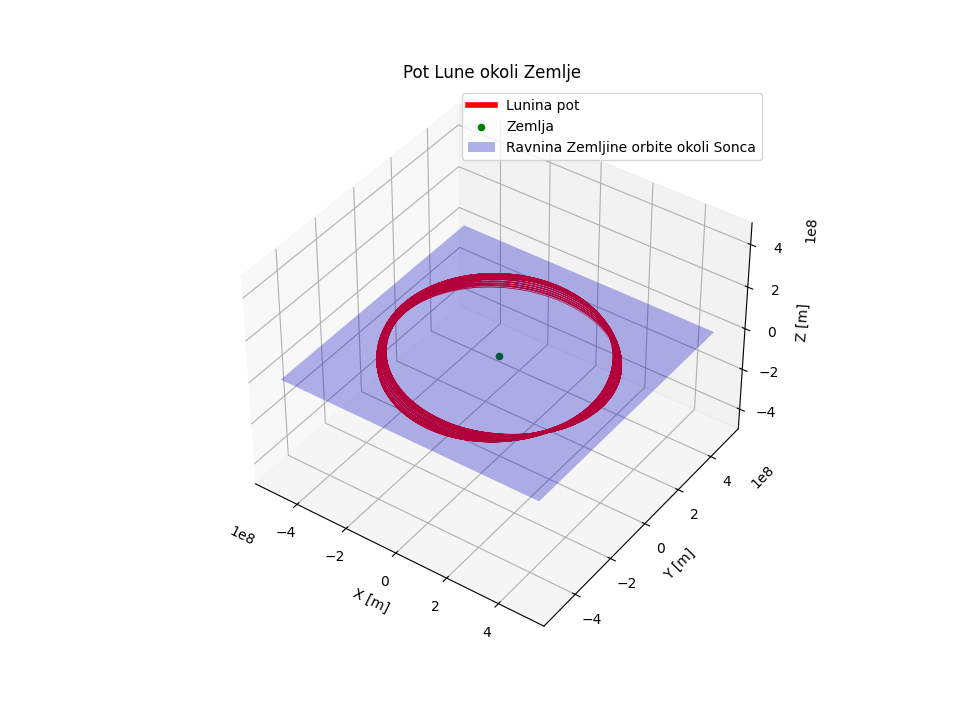
\includegraphics[scale=0.65]{Slike/Orbita_Lune_vseStrani.png}
\caption{Pot Lune okoli Zemlje}
\label{orb . Luna vse strani}
\end{center}
\end{figure}

\begin{figure}[H]
\begin{center}
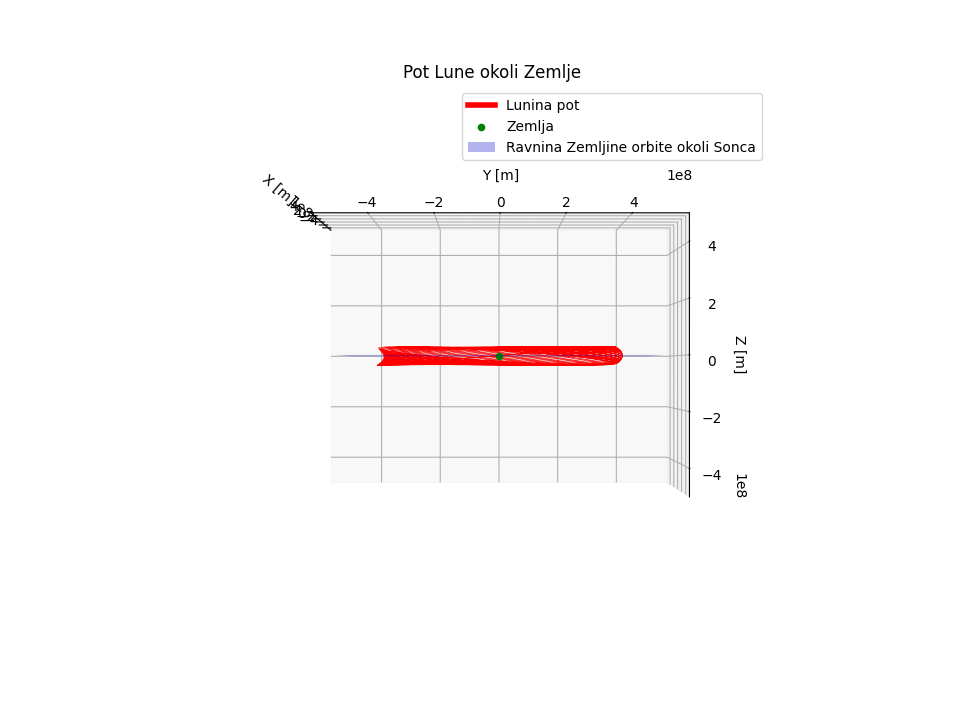
\includegraphics[scale=0.65]{Slike/Orbita_Lune_YZravnina.png}
\caption{Projekcija Lunine poti na YZ ravnino}
\label{orb . Luna YZ}
\end{center}
\end{figure}

Poglejmo še, ali se res spreminja položaj velike polosi.Zanima nas, kakšne so projekcije $\overrightarrow{r_{ZL}}$ vektorjev na XY ravnino. Če ne pride do spremembe položaja velike polosi, potem se projecirani vektorji ne bi smeli odstopati od projeciranih vektorjev prve orbite. Iz Slike \ref{orb. Luna XY} je razvidno, da pride do velikih odstopanj od prve orbite in da so orbite omejene z dvema elipsama.
\begin{figure}[H]
\begin{center}
	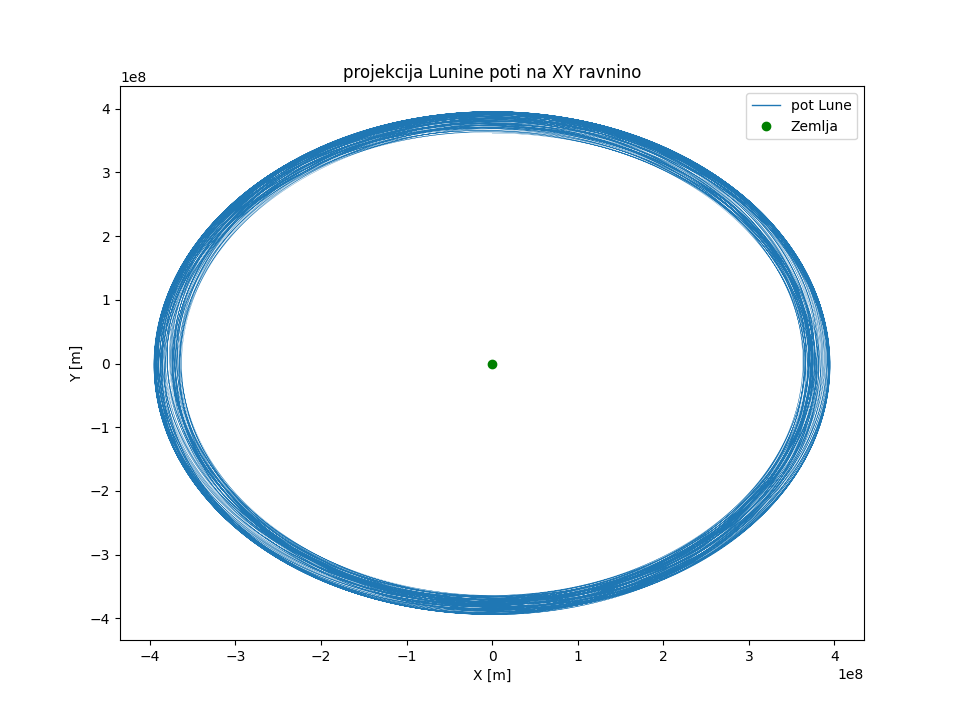
\includegraphics[scale=0.6]{Slike/Orbita_Lune_XYravnina}
	\caption{Projekcija Lunine poti na ravnino Zemljine orbite okoli Sonca}
	\label{orb. Luna XY}
\end{center}
\end{figure}

\subsection{Prva podnaloga}
Pri računanju kotov med ravninama, sem opazil, da je največji kot med ravninama večji, kot začeten kot  $\theta$. Dobil sem, da je največji kot med ravninama približno 5.40°. Prve sem povečal čas simulacije na približno 500 orbit. Nato sem kot med ravninama za vsako orbito vnesel v graf $\alpha(t)$ (Slika \ref{koti inklinacije v grafu}). Iz Slike \ref{koti inklinacije v grafu} se vidi, da se kot med ravninama spreminja periodično in spominja na funkcijo $cos(t)$. Opazimo tudi, da je čas ene periode zelo dolg (med 6000 in 8000 dnevi).

\begin{figure}[H]
\begin{center}
	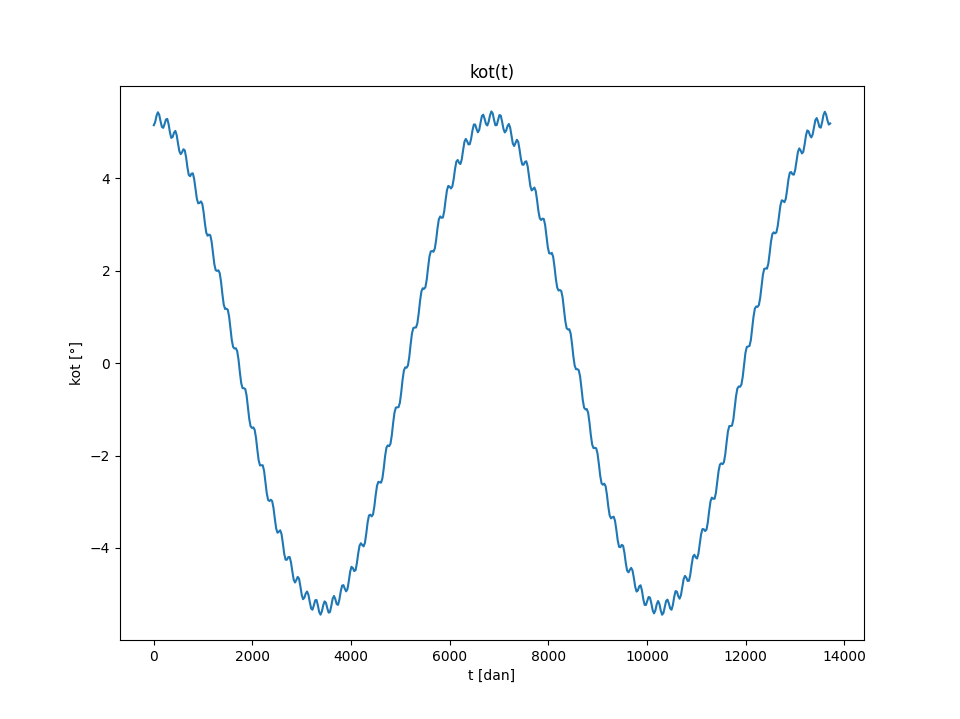
\includegraphics[scale=0.6]{Slike/inklinacija_kot_t}
	\caption{Kot med ravnino Lunine orbite okoli Zemlje in ravnine Zemljine orbite okoli Sonca.}
	\label{koti inklinacije v grafu}
\end{center}
\end{figure}

Ker nas zanima obhodni čas precesije kota ravnine Lunine orbite okoli Zemlje, sem na točke iz grafa $\alpha(t)$ z uporabo nelinearne regresije "fital"\ funkcijo $\alpha(t) = A cos(\omega_1 t)$, kjer sta $A$ in $\omega_1$ parametra, ki jih ne poznamo. Iz Slike  \ref{alfa(t) z fitano krivuljo} je vidno, da se taka oblika funkcije s pravimi parametri dobro prilega točkam $\alpha(t)$. Ker poznamo natančno  parametre "fitane"\ funkcije, lahko izračunamo obhodni čas precesije kota ravnine Lunine orbite okoli Zemlje po enačbi (\ref{obhodni čas}). Iz funkcije $\alpha(t)$ sem dobil, da je $\omega_1 = 9.183 \times 10^{-4}(dan)^{-1}$, kar pomeni, da je $t_0 = 18.73$ let. Dobljeni rezultat je od izmerjene vrednosti za 0.13 leta daljši. To pomeni, da je relativna napaka našega rezultata $0.7\%$. Napako sem izračunal glede na obhodne čase precesij dane na spletni strani \cite{Lun. preces.}.

\begin{figure}[H]
\begin{center}
	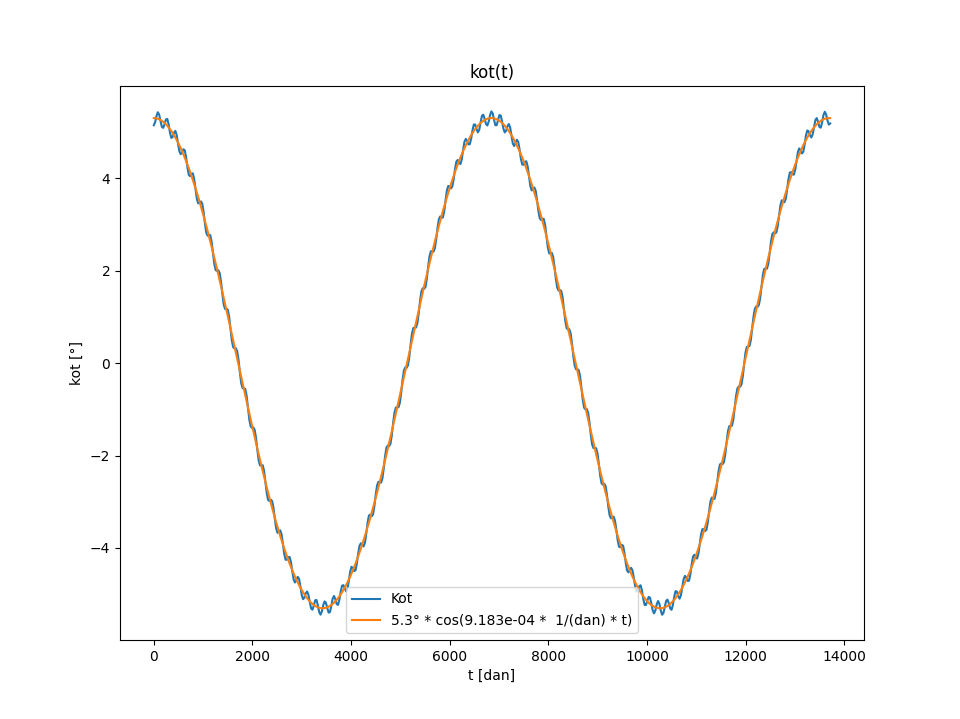
\includegraphics[scale=0.6]{Slike/inklinacija_kot_t_fitted}
	\caption{Točke $\alpha(t)$ in "fitano"\ funkcijo. "Fitana"\ funkcija :  $\alpha(t) = 5.3^{\circ}\ cos(9.183 \times 10^{-4}(dan)^{-1}\ t)$}
	\label{alfa(t) z fitano krivuljo}
\end{center}
\end{figure}

Enačba obhodnega časa :

\begin{large}
\begin{equation}
t_0 = \frac{2\pi}{\omega}
\label{obhodni čas}
\end{equation}
\end{large}

\subsection{Druga podnaloga}
Ker me zanima, kako se spreminja smer velike polosi, sem v graf $x(t)$ vnašal x komponento smeri velike polosi (Slika \ref{smer polosi}). Iz Slike \ref{smer polosi} je vido, da se smer velike polosi ne spreminja enakomerno v eno smer, vedar poskakuje, a ima nek trend vrtenja. Poleg tega se vidi, da je pojav periodičen, saj se trend vrtenja polosi nadaljuje tudi po prvem zavrtljaju smeri polosi.

\begin{figure}[H]
\begin{center}
	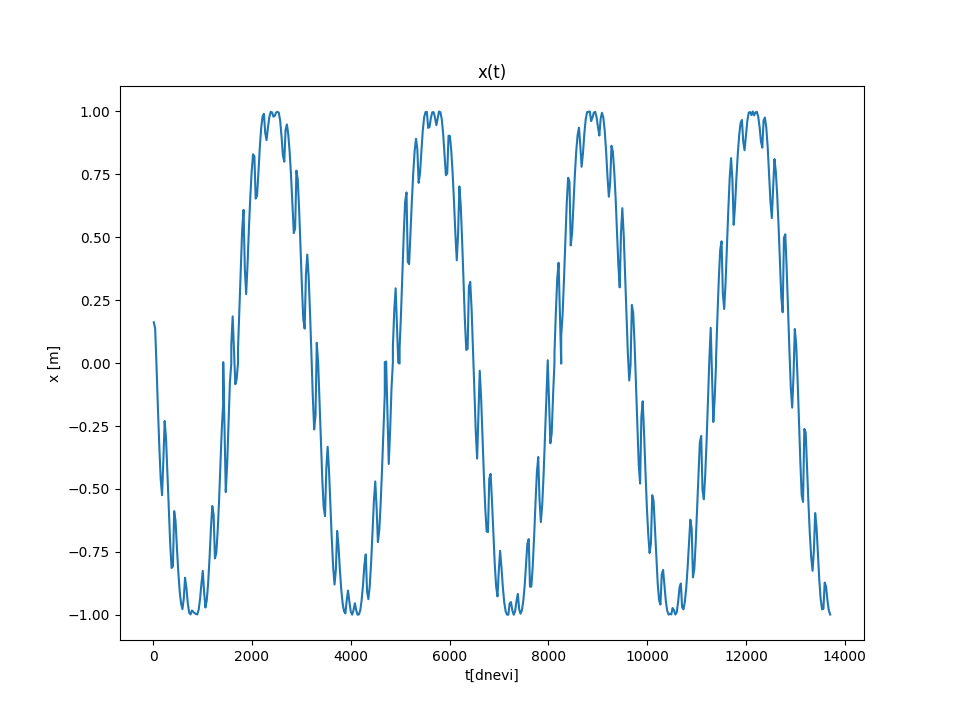
\includegraphics[scale=0.6]{Slike/smer_glavne_polosi}
	\caption{X komponenta vektorja smeri velike polosi elipse.}
	\label{smer polosi}
\end{center}
\end{figure}

Za izračun obhodnega časa precesije velike polosi lunine orbite, sem izbral podobno metodo, kot pri prvi podnalogi. Na graf $x(t)$ sem z pomočjo nelinearne regresije "fital"\ funkcijo $x(t) = -1 sin(\omega_2 t)$, kjer je $\omega_2$ parameter, ki ga ne poznamo. Iz Slike \ref{smer polosi fittano} se vidi, da se ta funkcija $x(t)$ s pravim parametrom dobro prilega podatkom in iz nje lahko izračunamo obhodni čas po enačbi (\ref{obhodni čas}). Iz "fitane"\ funkcije sem dobil, da je $\omega_2 = 1.940\times 10^{-3}(dan)^{-1}$, kar pomeni, da je $t_0 = 8.87$ let. Dobljeni rezultat je za 0.02 leta previsok. To pomeni, da je naša relativna napaka rezultata $0.2\%$. Napako sem izračunal glede na obhodne čase precesij dane na spletni strani \cite{Lun. preces.}.

\begin{figure}[H]
\begin{center}
	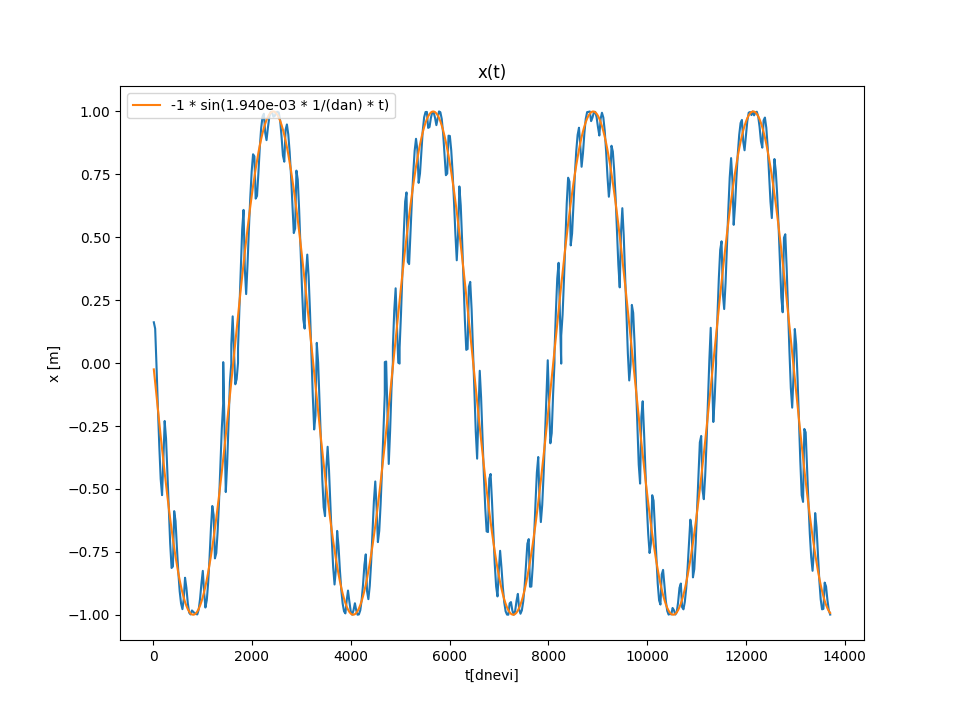
\includegraphics[scale=0.6]{Slike/smer_glavne_polosi_fitted}
	\caption{Točke $x(t)$ in "fitana"\ funkcija. "Fitana funkcija"\ : $x(t) = -1sin(1.940\times 10^{-3}(dan)^{-1}t)$}
	\label{smer polosi fittano}
\end{center}
\end{figure}

\subsection{Zanimivost}
Pri numeričnem integriranju sem opazil, da začetni pogoji zelo vplivajo na končen rezultat. Na primer, če samo spremenimo smer začetne hitrosti Zemlje za $180^{\circ}$ dobimo čas precesije kotov med ravninama orbit drugačen ($t_0$ pride približno 17.5 let). Poleg tega je spreminjanje smeri glavne polosi popolnoma drugačno, kar je razvidno na Sliki \ref{smer polosi obratna smer}.

\begin{figure}[H]
\begin{center}
	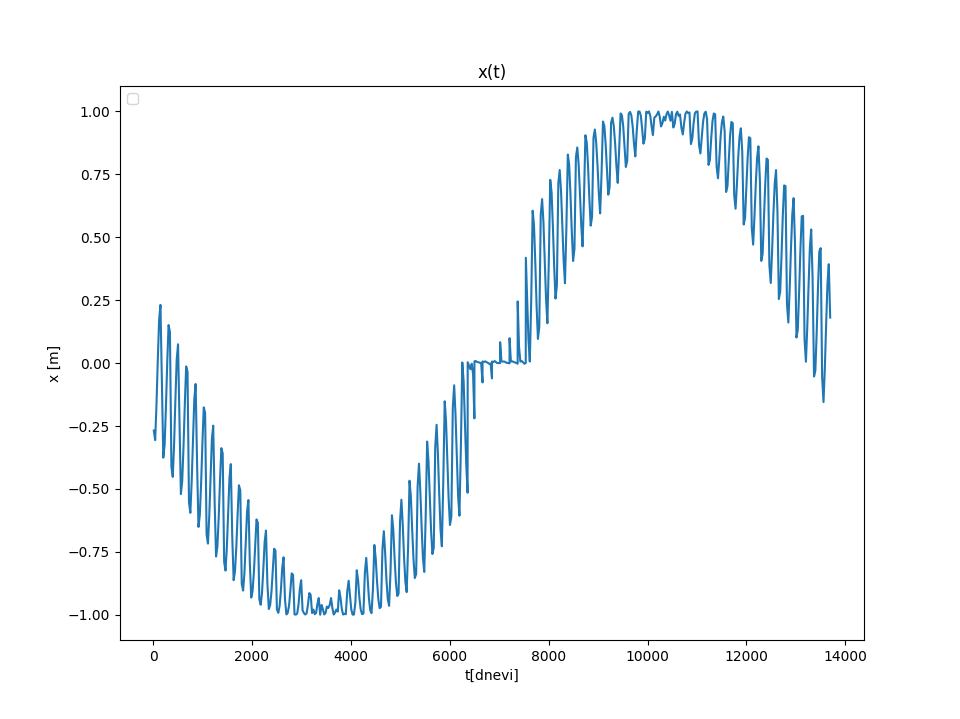
\includegraphics[scale=0.6]{Slike/obratna_smer_x_t}
	\caption{Točke $x(t)$, če se Zemlja vrti okoli Sonca v obratni smeri}
	\label{smer polosi obratna smer}
\end{center}
\end{figure}

\section{Zaključek}
S pomočjo numeričnega integriranja sem simuliral Lunino pot okoli Zemlje in izračunal precesijo kota med ravnino Lunine orbite okoli Zemlje  in ravnino Zemljine orbite okoli Sonca ter precesijo vrtenja velike polosi  Lunine eliptične orbite. Obhodni čas precesije kota med ravnino Lunine orbite okoli Zemlje  in ravnino Zemljine orbite okoli Sonca sem dobil 18.73 let. Obhodni čas precesije vrtenja velike polosi  Lunine eliptične orbite sem dobil 8.87 let. Izračunane vrednosti se od izmerjenih vrednosti razlikujejo za manj kot 1\%, kar pomeni, da je bilo numerično integriranje uspešno. Poleg tega sem ugotovil, da je je obhodni čas obeh precesij odvisen od smeri kroženja okoli nebesnega telesa in da je največji kot med ravninama orbit Zemlje okoli Sonca in Lune okoli Zemlje večji od podanega v \cite{Zak nal}. Rezultati, ki sem jih dobil, se ne razlikujejo veliko od pričakovanih izmerjenih rezultatov. Mislim, da bi se rezultati še bolje prilegali pričakovanim vrednostim, če bi naš sistem razširili in upoštevali tudi vpliv drugih planetov v osončju še posebaj vpliv Jupitra, ker je najtežji planet v osončju.

\begin{thebibliography}{99}

	\bibitem{Zak nal} D. Svenšek, Zaključna naloga 2023/24. \url{https://predmeti.fmf.uni-lj.si/racorodja?action=AttachFile& do=get& target=08_zakljucna_naloga.pdf}
	\bibitem{Luna} Moon Fact Sheet. \url{https://nssdc.gsfc.nasa.gov/planetary/factsheet/moonfact.html}
	\bibitem{Zemlja} Earth Fact Sheet. \url{https://nssdc.gsfc.nasa.gov/planetary/factsheet/earthfact.html}
	\bibitem{Sonce} The Sun. \url{https://www.mccc.edu/~dornemam/Planet_Walk/Sun/the_sun.htm}
	\bibitem{Lun. preces.} Lunar Precession. \url{https://en.wikipedia.org/wiki/Lunar_precession}

\end{thebibliography}

\end{document}
